% ============================================================
% Q3: Multidimensional Attribution Analysis (compressed, O-level)
% Keep existing figures Q3.1--Q3.4
% ============================================================

\section{Quantifying Judges' and Audience Impacts on Elimination Risk}

\label{sec:q3}

\subsection{Latent Uncertainty Propagation to Downstream Models }
\label{sec:q3_inputs}

To propagate the uncertainty inherent in the inverse reconstruction, we bypass deterministic point estimates and instead utilize the full posterior ensemble $\{\mathbf v^{(m)}_{s,t}\}_{m=1}^{M}$ ($M=2000$), where each $\mathbf v^{(m)}_{s,t}$ satisfies the simplex constraint $\sum_{i\in C_{s,t}} v^{(m)}_{i,s,t}=1$. By treating each draw as a completed popularity scenario and pooling downstream estimates via Rubin's multiple-imputation rules , we ensure that subsequent analyses reflect the true ambiguity of the latent votes rather than the bias of plug-in means.
\paragraph{Pooling rule (Rubin's MI).}
Let $\theta^{(m)}$ denote an estimate computed under draw $m$ with estimated variance $U^{(m)}$ (e.g., from the fitted model). Rubin's rules pool uncertainty as
\[
\bar\theta=\frac{1}{M}\sum_{m=1}^M \theta^{(m)},\quad
\bar U=\frac{1}{M}\sum_{m=1}^M U^{(m)},\quad
B=\frac{1}{M-1}\sum_{m=1}^M\left(\theta^{(m)}-\bar\theta\right)^2,\quad
T=\bar U+\left(1+\frac{1}{M}\right)B,
\]
and we report $\bar\theta\pm 1.96\sqrt{T}$ when approximate normality is adequate.


\begin{definition}[Attribution Challenge]
Elimination outcomes are driven by heterogeneous channels: a meritocratic channel (judges) and a democratic channel (fans).
The attribution challenge is to quantify the conditional contribution of professional partners after controlling for celebrity traits and season-week context,
without extrapolating counterfactual post-elimination trajectories.
\end{definition}

\begin{definition}[Meritocratic Signal]
For $i\in C_{s,t}$, the observed judge input is $J_{i,s,t}$ (field \texttt{wt\_avg}).
Define within-week standardized judge performance
\[
Y^J_{i,s,t}=\frac{J_{i,s,t}-\bar J_{s,t}}{\sigma_{J,s,t}},\qquad
\bar J_{s,t}=\frac{1}{|C_{s,t}|}\sum_{k\in C_{s,t}}J_{k,s,t},
\]
where $\sigma_{J,s,t}$ is the sample standard deviation of $\{J_{k,s,t}:k\in C_{s,t}\}$.
\end{definition}

\begin{definition}[Democratic Signal in Euclidean Geometry]
For each draw $m$, fan support lies on the simplex and is mapped to Euclidean space by the centered log-ratio (CLR). To ensure the log transform is well-defined, we apply a machine-level pseudocount and renormalize:
\[
v^{\dagger(m)}_{i,s,t}=\max\{v^{(m)}_{i,s,t},\epsilon\},\qquad
\tilde v^{(m)}_{i,s,t}=\frac{v^{\dagger(m)}_{i,s,t}}{\sum_{k\in C_{s,t}} v^{\dagger(m)}_{k,s,t}}.
\]
We then compute
\[
\mathrm{clr}\!\left(\tilde v^{(m)}_{i,s,t}\right)=
\log \tilde v^{(m)}_{i,s,t}-\frac{1}{|C_{s,t}|}\sum_{k\in C_{s,t}}\log \tilde v^{(m)}_{k,s,t}.
\]

Define within-week standardized popularity response
\[
Y^{V(m)}_{i,s,t}=
\frac{\mathrm{clr}(v^{(m)}_{i,s,t})-\overline{\mathrm{clr}}^{(m)}_{s,t}}{\sigma^{(m)}_{\mathrm{clr},s,t}},
\]
so that $Y^{V(m)}_{i,s,t}$ and $Y^{J}_{i,s,t}$ are comparable on a one-standard-deviation scale.
\end{definition}

To isolate the impact of professional partners while strictly preventing data leakage, we construct a \textbf{Leakage-Controlled Pro Profile} $\mathbf z_{d,s}=(\mathrm{Tenure}_d,\ \mu^{J,\mathrm{LOSO}}_{d,-s})^\top$, where $\mu^{J,\mathrm{LOSO}}_{d,-s}$ represents the partner's historical performance averaged over all seasons $s'\neq s$ (a \textbf{Leave-One-Season-Out} estimator). Simultaneously, we account for contestant heterogeneity via \textbf{Celebrity Covariates} $\mathbf x_i$, comprising centered age and stabilized industry dummies (with rare categories merged into \texttt{Other}).

\subsection{The Judge-Fan-Survival Three-Channel Architecture }
\label{sec:q3_models}

To disentangle the mechanisms conflated in the raw elimination outcomes, we structurally model three distinct components: the judges' technical assessment, the fan preference conditional on observed performance, and the stochastic advancement dynamics governing the risk set.

\paragraph{Channel J: technical assessment (judges).}
Let $Y^J_{i,s,t}$ be the within-week standardized judge score. We use a mixed-effects structure that isolates (a) celebrity traits, (b) interpretable pro profile effects, and (c) residual partner heterogeneity:
\begin{equation}
Y^J_{i,s,t}
=
\mathbf x_i^\top \boldsymbol\beta^J
+
\mathbf z_{d(i),s}^\top \boldsymbol\eta^J
+
\phi_{\mathrm{era}(s),t}
+
u_s^J
+
b^J_{d(i)}
+
\epsilon^J_{i,s,t}.
\label{eq:q3_judge_lmm}
\end{equation}
\noindent\textbf{Notation (model components).}
$\mathbf x_i$ are celebrity covariates; $d(i)$ maps celebrity $i$ to professional partner $d$; $\mathbf z_{d(i),s}$ is the leakage-controlled pro profile; $\phi_{\mathrm{era}(s),t}$ is an era-by-week fixed effect; $u_s^{J/V}$ are season random intercepts; $b_{d}^{J/V}$ are pro-dancer random effects; $\epsilon$ are idiosyncratic errors; and $\kappa_J,\kappa_V$ quantify the protective effects of technical merit and popularity in the hazard.


\paragraph{Channel V: popularity conditional on performance (fans).}
For each draw $m$, let $Y^{V(m)}_{i,s,t}$ denote the standardized log-ratio popularity response. Conditioning on contemporaneous performance prevents ``good dancing'' from being misread as ``being liked'':
\begin{equation}
Y^{V(m)}_{i,s,t}
=
\mathbf x_i^\top \boldsymbol\beta^V
+
\mathbf z_{d(i),s}^\top \boldsymbol\eta^V
+
\gamma\, Y^J_{i,s,t}
+
u_s^V
+
b^V_{d(i)}
+
\epsilon^{V(m)}_{i,s,t}.
\label{eq:q3_fan_lmm}
\end{equation}

\paragraph{Channel H: advancement dynamics (discrete-time survival).}
Let $h^{(m)}_{i,s,t}$ be the elimination hazard at week $t$ given survival to $t{-}1$.
A discrete-time hazard specification links advancement to both technical and popularity signals\footnote{Discrete-time hazard modeling follows standard survival texts.}:
\begin{equation}
\mathrm{logit}\!\left(h^{(m)}_{i,s,t}\right)
=
\delta_t
+
\mathbf x_i^\top \boldsymbol\beta^H
+
\kappa_J\, Y^J_{i,s,t}
+
\kappa_V\, Y^{V(m)}_{i,s,t}.
\label{eq:q3_hazard}
\end{equation}
where $\delta_t$ is the week-specific baseline log-odds (time effect).

\subsection{Visual Analysis of Findings and Robustness Checks }
\label{sec:q3_findings}

Crucially, our analysis reveals that \textbf{Fan and Judge Criteria} decouple along interpretable dimensions (Figure~\ref{fig:q3_coef_contrast}). While technical scoring exhibits a sharp negative gradient with age, conditional fan preference is attenuated and frequently reverses direction. This divergence provides quantitative evidence of a \textbf{Sympathy-Compensation Pattern}, where audience support actively counterbalances technical deficits rather than purely tracking performance.

\begin{figure}[t]
  \centering
  \begin{subfigure}[t]{0.53\textwidth}
    \centering
    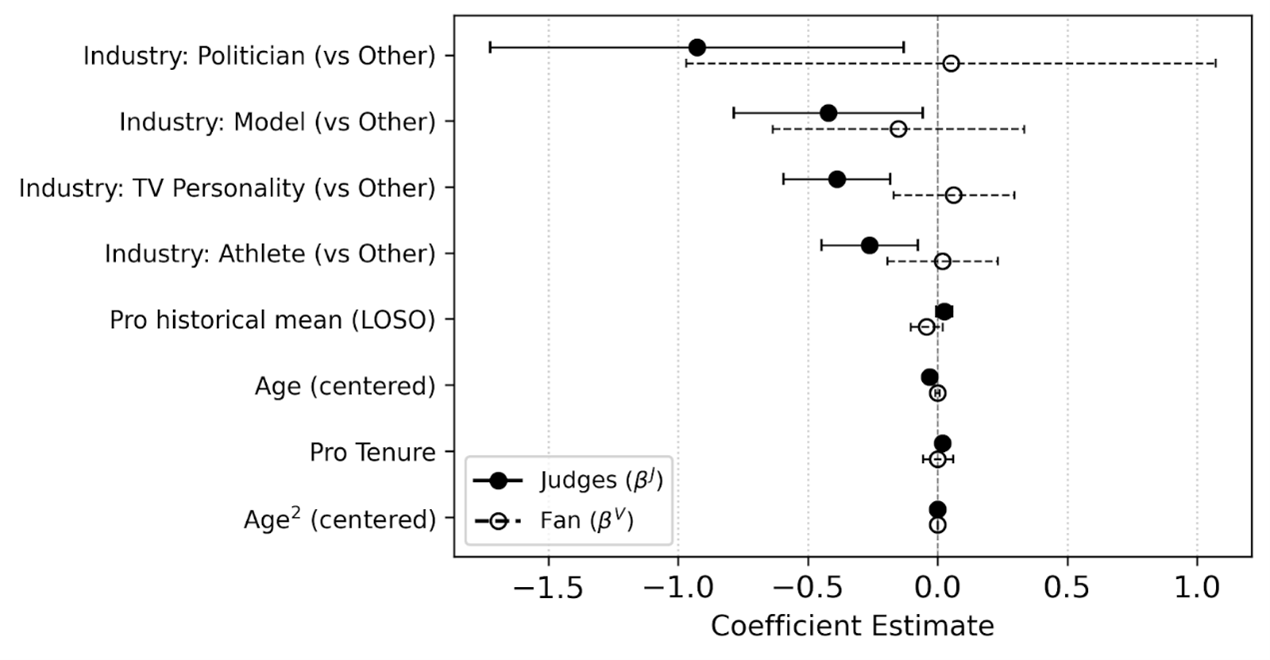
\includegraphics[width=\textwidth]{figures/Q3.1.png}
    \caption{Fixed-effect estimates (standardized) with 95\% intervals for the judge channel ($\boldsymbol\beta^J$) and the fan channel ($\boldsymbol\beta^V$), with fan-side uncertainty pooled over $M=2000$ Q1 posterior vote draws.}
    \label{fig:q3_coef_contrast}
  \end{subfigure}
  \hfill
  \begin{subfigure}[t]{0.43\textwidth}
    \centering
    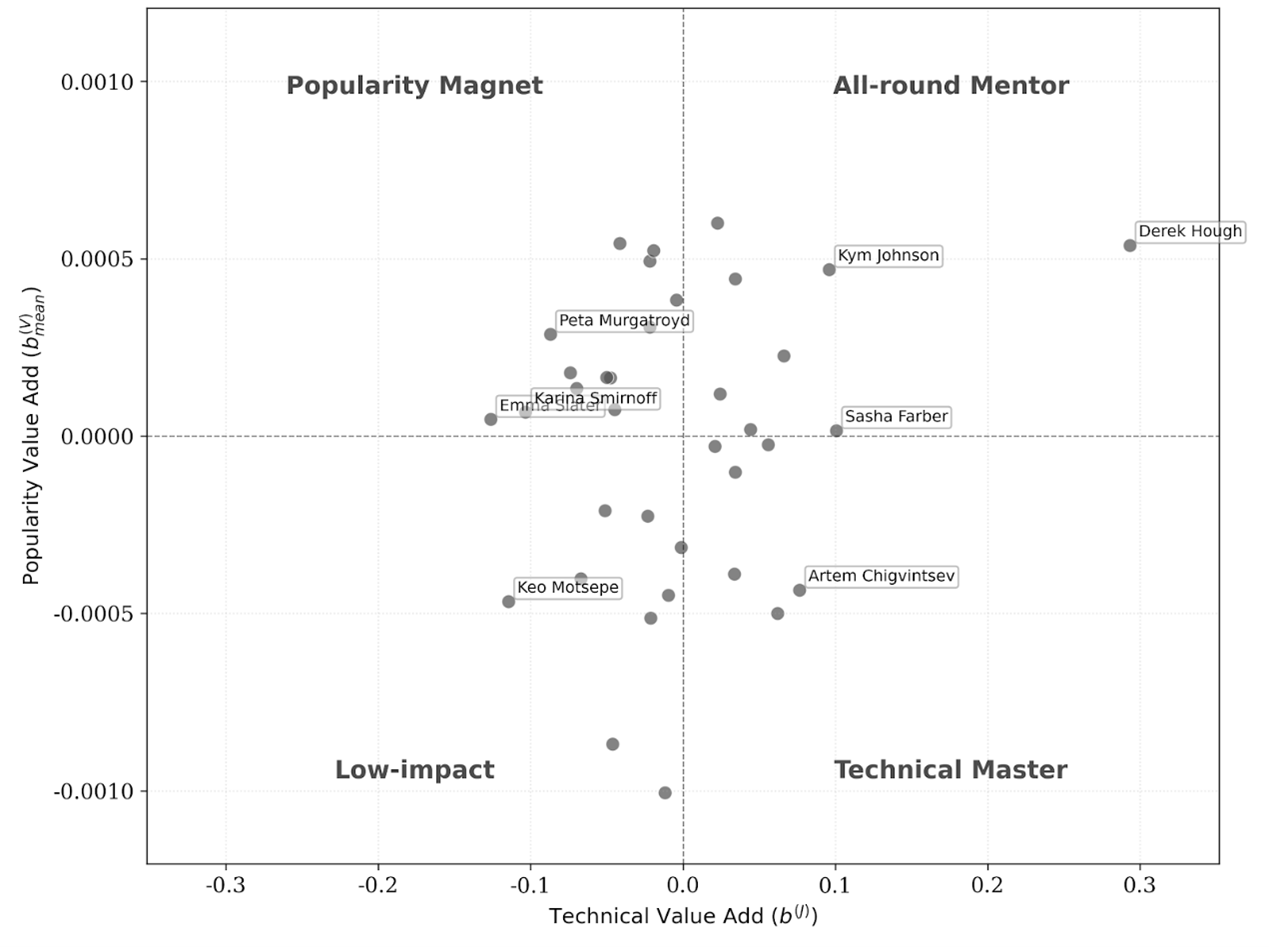
\includegraphics[width=\textwidth]{figures/Q3.2.png}
    \caption{Each professional is positioned by estimated residual technical value add ($b^{(J)}$) and residual popularity value add ($b^{(V)}$), separating ``technical uplift'' from ``popularity transfer'' beyond observed covariates.}
    \label{fig:q3_pro_scatter}
  \end{subfigure}
  \caption{\textbf{Cross-channel contrast and pro-dancer value add.}}
  \label{fig:q3_side_by_side}
\end{figure}


Furthermore, Figure~\ref{fig:q3_pro_scatter} demonstrates that professional partner effects are strongly \textbf{Channel-Dependent}, distinguishing technical specialists (positive $b^{(J)}$) from popularity multipliers (positive $b^{(V)}$) and revealing a heterogeneous ``value add'' that transcends simple tenure metrics.



Finally, the hazard estimates in Fig.~\ref{fig:q3_or_forest} corroborate that advancement is governed by a robust \textbf{Dual-Signal Mechanism}. Both technical merit ($Y^J$) and audience support ($Y^{V(m)}$) exert significant protective effects, confirming that elimination remains a joint decision process even after adjusting for demographic covariates and baseline weekly risk.

\begin{figure}[H]
  \centering
  \begin{subfigure}[t]{0.43\textwidth}
    \centering
    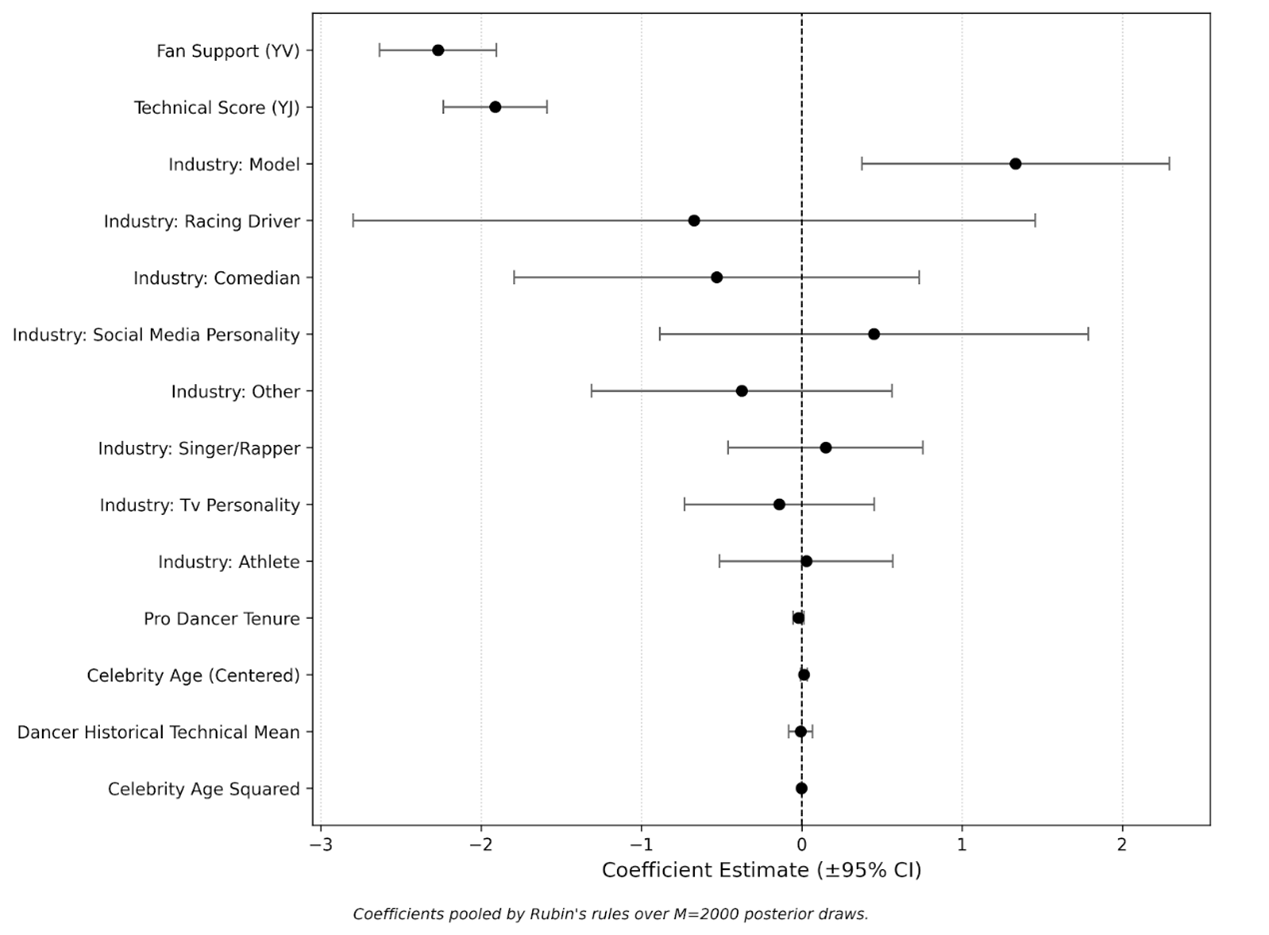
\includegraphics[width=\textwidth]{figures/Q3.3.png}
    \caption{Coefficients with 95\% intervals pooled over $M=2000$ Q1 posterior vote draws.}
    \label{fig:q3_or_forest}
  \end{subfigure}
  \hfill
  \begin{subfigure}[t]{0.53\textwidth}
    \centering
    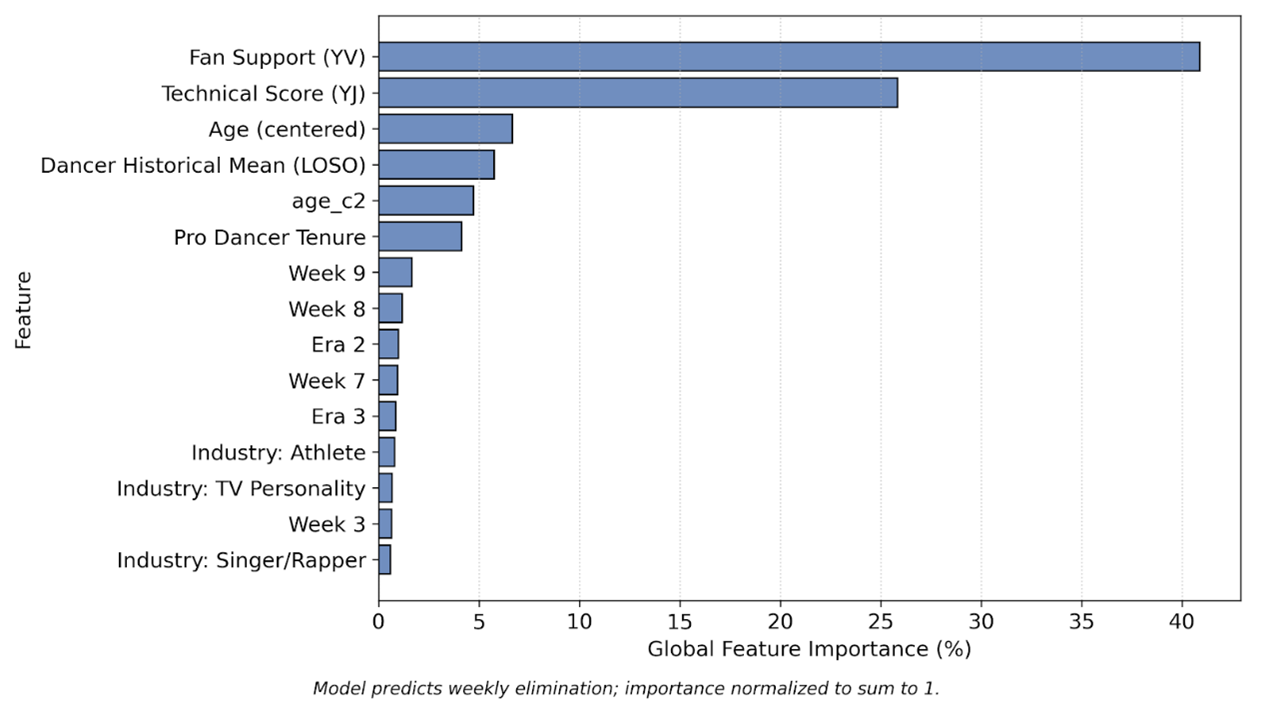
\includegraphics[width=\textwidth]{figures/Q3.4.png}
    \caption{Random forest analysis confirms the primacy of performance and fan support over secondary demographic factors.}
    \label{fig:q3_rf_importance}
  \end{subfigure}
  \caption{\textbf{Determinants of survival and robustness diagnostics.}}
  \label{fig:q3_survival_and_rf}
\end{figure}

To corroborate this driver hierarchy, we employ a nonparametric \textbf{Random Forest} diagnostic (Fig.~\ref{fig:q3_rf_importance}). The resulting importance scores confirm that elimination risk is dominated by contemporaneous performance and fan support, relegating age and professional attributes to secondary yet systematic roles\footnote{Random forests serve here solely as a robustness diagnostic .}.

Refining the functional form reveals Nonlinear Age Effects, where a quadratic specification yields a U-shaped risk profile, implying practical limits to sympathy compensation. Regarding identification, we acknowledge Matching Endogeneity due to non-random partner assignment; we therefore interpret estimates as conditional associations, utilizing Leakage-Controlled Pro Profiles to mitigate selection bias in the absence of an external instrument.







